\chapter{ Basic Scattering Theory}
\section{Remarks on the quantum scattering theory}
Scattering problem in quantum theory is a vast topic, it is the second problem in quantum mechanics along with bounded states one. There are two main cases for a an interacting quantum particle; the first is when it's \textbf{bounded to a potential}. The particle takes a \textbf{discrete energy spectrum }. The second case, is when the particle is \textbf{scattered of a potential}, and takes a c\textbf{continuous spectrum of energy}.\\  Hence, we inscribe the incident wavefunction $ ^o \psi(x,t)$ by a free particle wave-packet ( as plane wave). The scatterer, is a stationary potential, that elastically scatter off the incident wave-packet ( in our simplified problem), i.e. the energy is conserved.
\begin{figure}[h!]
	\centering
	\label{scat}
	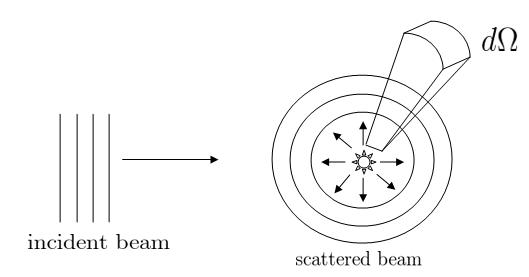
\includegraphics[scale=0.6]{./figures/Scattering}
	\caption{Sketch of the scattering problem in quantum mechanics. Notice that we use the wave nature of the quantum particles} 
\end{figure}
Then the scattered wave shall be a spherical wavefunction $^{out} \psi(\vec{r},t)$, we care about the probability for a scattering with a certain solid angle $\Omega$. This is calculated from the\textbf{ differential cross-section} see figure \ref{scat}:
\begin{equation}
\frac{d \sigma}{d \Omega}\equiv \frac{N_{\phi ,\theta}}{^oj}
\end{equation}
Where $N_{\phi ,\theta}$ is the probability of detecting the scattered particle by a detector placed at angles $ \phi$ and $ \theta$ . And $ ^oj$ is the incident probability flux current. i.e:
\begin{equation}
^oj = \frac{\hbar}{2mi} \left( ^o \psi(x,t)^* \frac{\partial ^o \psi(x,t)}{\partial x}- ^o \psi(x,t) \frac{\partial ^o \psi(x,t)^*}{\partial x}\right) 
\label{current}
\end{equation} 
However, we shall restrict ourselves to one dimensional scattering problems, where the differential cross section calculation is not the major problem. Rather we are interested in the probability of transmission and reflection of the incident flux. 
\section{Scattering/Reaction channels}
In general, for two particles $a$ and $b$ interacting in a scattering problem. We have many possible \textbf{reaction channels}; listed as follows:
\begin{table}[h!]
	\centering
	\begin{tabular}{|l|c|}
		\hline
		Reaction channel& Name\\
		\hline
		$a+b$  $\longrightarrow$  $ a+b$ & Elastic scattering \\
		$a+b$  $\longrightarrow$  $ a+b^*$ & Inelastic scattering \\
		$a+b$  $\longrightarrow$  $ c+d$ & Rearrangement collision \\
		$a+b$  $\longrightarrow$  $ c$ & Absorption \\
		$a$  $\longrightarrow$  $ b+c$ & Decay\\
		\hline
	\end{tabular}
	\caption{Classification of the reaction channels in a tow-particle scattering problem}
\end{table}
\section{Scattering by potentials in 1-D}
A moving wave-packet with an energy $E$ approaching some potential variations illustrated in figure . Will have the general solution for their time-independent Schr\"{o}dinger equation  (TISE):
\begin{subequations}
	\begin{align}
	\psi_L (x)&=Ae^{+ikx}+Be^{-ikx} \\
	\psi_R (x)&=Ce^{+ikx}+De^{-ikx} 
	\end{align}
	With:
	\begin{equation}
	k^2= \frac{2mE}{\hbar^2} \nonumber 
	\end{equation}
\end{subequations}
The previous set of equations can be put in a vector form as follows:
\begin{equation}
^{out}\Psi = S\cdot ^{o}\Psi \; \; \; \;  \Leftrightarrow \begin{pmatrix}B \\ C \end{pmatrix} = \begin{pmatrix} S_{11} & S_{12} \\ S_{21} & S_{22} \end{pmatrix}\begin{pmatrix} A \\ D \end{pmatrix}.
\end{equation}
This equation resembles the scattering amplitude and $S$ is known as the \textbf{S-matrix}, and it plays an important r\^{o}le in scattering problems. As the S-matrix elements characterises the full properties of the scattering process.\\ Recall the current density in \eqref{current} is conserved, i.e.:
\begin{equation}
j_R= j_L
\end{equation}
That implies:
\begin{equation}
|A|^2 -|B|^2 = |C|^2-| D|^2
\end{equation}
Since:
\begin{subequations}
	\begin{align}
	j_L =& \frac{\hbar k}{m}\left( |A|^2 -|B|^2\right)  \\
	j_R =& \frac{\hbar k}{m}\left( |C|^2 -|D|^2\right)
	\end{align}
\end{subequations}
Since we have in our problem the incident flux is from the left only $ \Rightarrow D=0$. We have thereby:
\begin{align*}
T_L&= \left| \frac{C}{A}\right|^2 = |S_{21}|^2  &  R_L&= \left| \frac{B}{A}\right|^2 = |S_{11}|^2
\end{align*}
Or similarly for flux approaching from right $ A=0$ :
\begin{align*}
T_R&= \left| \frac{B}{B}\right|^2 = |S_{12}|^2  &  R_R&= \left| \frac{C}{D}\right|^2 = |S_{11}|^2
\end{align*}
With $T$ and $R$ are the transmission and reflection probabilities respectively. \\ Note that:
\begin{equation}
T_{L (R)} +R_{L(R)} = 1
\end{equation}
\section{The optical theorem in 1-D}
Consider a free particle $ (V =0) $, we can write the its S-matrix as:
\begin{equation}
S = \begin{pmatrix}
0&1\\1&0
\end{pmatrix},
\end{equation}
taking the canonical form. When $ (V\neq 0)$, $S$ should be written according to the continuity conditions. Let :
\begin{align}
\psi(x)_L& = e^{i kx}+ r e^{-ikx}  & \psi(x)_R &= te^{ikx}
\end{align}
Satisfying the conditions ( $V$ changes at $ x=0$):
\begin{align}
\psi(x= 0)_L& = \psi(x=0)_R  &  \frac{d \psi(x)_L}{dx}| _{x=0} &= \frac{d \psi(x)_R}{dx}| _{x=0}
\end{align}
We obtain the expression for the S-matrix:

\begin{equation}
S = \begin{pmatrix}
2ir&1+2it\\1+2it&2ir^* \frac{1+2it}{1-2it^*}
\end{pmatrix},
\end{equation}
Or:
\begin{equation}
\boxed{|r|^2+|t|^2 = \Im(t)}
\end{equation}
Which is \textbf{the optical theorem } in one dimension.


\nocite{*} 